% REVISION: 2026-08-09 r17 -- task-17 folded in: Sec.2 r3 exception
%   (candidates with no accelerator-side generative instance record
%   y3=0; per-view rates not retained); App.B prediction-path sentence
%   (regressor scores every candidate, beta per set, harmless -- S3 all
%   correct); App.F FACT FIX: previous "selected max_depth=5, eta=0.1"
%   was wrong (not in grid); replaced with actual grid
%   {(3,.1),(4,.1),(5,.05),(6,.1)}, inner 3-fold group-aware CV, MAE
%   selection, fixed params. Pending: Contribution (iii)+conclusion
%   decision; fit; deck sync; mirror/zip.
% REVISION: 2026-08-09 r16 -- ChatGPT round-2 accepted items applied to
%   author base (which already carried Table-1 greedy cell denominators):
%   abstract scope qualifier (platform-wise group-normalized, controlled
%   phrase removed -- title carries it); Sec.4 divergence qualified via
%   Eq.~ref; App.H repeated-measurement claim corrected; App.A
%   verifies->examines whether; App.C beta-claim replaced by platform-
%   difference conclusion (alpha-marginal kept; NOTE deck slide 12 has
%   the same overclaim -- fix at deck sync); Table 1 caption /45 bounds;
%   App.D raw Oracle-ratio column DELETED + definition rewritten;
%   Uncollected->Unmeasured; warm-up; App.G seed 20260715.
%   NOT applied (pending author): Contribution (iii) + conclusion
%   rewrite; r3 CPU-only sentence (task 17); App.F grid detail (task 17).

\documentclass{article}

\PassOptionsToPackage{numbers,sort&compress}{natbib}
\usepackage[dblblindworkshop, final]{neurips_2026}

\usepackage[utf8]{inputenc}
\usepackage[T1]{fontenc}
\usepackage{hyperref}
\hypersetup{hidelinks}
\usepackage{url}
\usepackage{booktabs}
\usepackage{amsmath,amssymb,amsfonts}
\usepackage{graphicx}
\usepackage{multirow}
\usepackage{xcolor}
\usepackage{enumitem}
\usepackage{caption}

% pack floats tightly on text pages
\setcounter{topnumber}{3}
\setlength{\textfloatsep}{5pt plus 1pt minus 2pt}
\renewcommand{\topfraction}{0.95}
\renewcommand{\textfraction}{0.03}
\renewcommand{\floatpagefraction}{0.9}
\setlength{\abovecaptionskip}{2pt}

% discourage mid-word line breaks; forbid breaks inside inline math
\hyphenpenalty=4000
\exhyphenpenalty=2000
\tolerance=1800
\emergencystretch=2.5em
\relpenalty=10000
\binoppenalty=10000

% ---- placeholder macros: MUST be empty of red before submission ----
\newcommand{\RES}[1]{\textcolor{red}{\textbf{#1}}}
\newcommand{\TODO}[1]{\textcolor{red}{[TODO: #1]}}

\workshoptitle{ML for Systems}
% \title{Divergent Placements, Unified Predictors:\\ A Controlled GPU/NPU Study of Multi-Model Inference Placement}

\title{Divergent Placements, Unified Predictor: A Controlled GPU and NPU Study of Multi-Model Inference}

\author{%
  Misun Yu\\
  Electronics and Telecommunications Research Institute\\
  \texttt{msyu@etri.re.kr}
  % \And  \TODO{co-authors}
}

\begin{document}

\maketitle

\begin{abstract}
Placing concurrent inference workloads on heterogeneous nodes is difficult because isolated profiles do not capture co-execution interference. We present a learning-based method that predicts system-level performance from offline profiles and ranks placements without online execution. Under our platform-wise group-normalized objective, the best measured placement differs between the GPU and NPU in 11 of 45 workload groups, including 10 involving generative models. Motivated by this accelerator-dependent behavior, we compare predictor performance under three settings: platform-specific training, zero-shot cross-accelerator transfer, and joint training on both platforms. Zero-shot transfer reduces ranking quality, whereas the jointly trained predictor approaches platform-specific performance. It matches the platform-specific predictors' Top-1 accuracies of 93.3\% on the GPU and 86.7\% on the NPU. In this two-platform evaluation, accelerator-specific profiling data improves ranking, while one jointly trained predictor supports both platforms.
\end{abstract}


\section{Introduction}
\label{sec:intro}

Modern inference nodes serve several applications on shared accelerators---detection and classification pipelines alongside language and vision-language models. Under co-execution these contend for the accelerator, host-side pipeline stages, and interconnect bandwidth, so a placement that is best in isolation is often not best under load. Contention is non-additive, so isolated profiles do not reliably predict concurrent behavior, and online evaluation is impractical because the candidate space grows exponentially with the number of workloads.

Learning-based models predict performance under contention~\citep{kim_iccd2024_interference,xu_tpds2023_igniter,cui2021}, but prior predictors are developed and evaluated on a single platform, leaving unclear whether they capture workload characteristics or accelerator-specific behavior. We study this question using a controlled two-platform testbed. The host configuration, nine-model suite, workload schedules, request rates, and 37-dimensional feature representation are held fixed. The accelerator platform is either an NVIDIA RTX~5090 GPU or a Mobilint MLA100 NPU~\citep{mobilint_mla100}. We collect 540 profiling windows per platform; XGBoost regressors are fitted on training folds only, and a tunable scoring function converts their predictions into a complete ranking of placement candidates without online measurement.

% The controlled comparison yields three findings. First, the placement with the highest measured score differs between the GPU and NPU in 11 of 45 workload groups. This difference occurs in 10 of 33 groups containing a generative model, compared with only 1 of 12 vision-only groups. Changes to the scoring weights also affect the best placement more often on the NPU than on the GPU. Second, a predictor trained on one accelerator transfers only partially to the other when used without retraining. We refer to this setting as zero-shot transfer. A predictor trained jointly on both platforms performs comparably to separate per-platform predictors. Supporting a new accelerator therefore requires additional profiling data, but not a separately maintained model. Third, direct system-level regression outperforms both a capacity-based greedy heuristic and an attainment-based per-instance decomposition~\citep{kim_iccd2024_interference}. The greedy heuristic achieves Top-1 accuracy of only 0.42 on the GPU and 0.33 on the NPU. The decomposed model predicts individual application performance accurately, but loses accuracy when combining these predictions into system-level metrics.

\textbf{Contributions.} (i) We formulate placement as a deployment-time measurement-free ranking problem after offline profiling, and evaluate it with group-wise cross-validation. (ii) We build a controlled GPU/NPU testbed with fixed host configuration, workloads, request rates, and features. (iii) We show that best measured placements and profiling data are accelerator-specific, while a jointly trained predictor performs comparably to separate platform-specific predictors. (iv) We compare direct regression with a capacity-based heuristic and an attainment-based decomposition. The advantage over the latter is statistically significant on the NPU but not on the GPU.


\section{Problem Formulation and Testbed}
\label{sec:problem}

Offline profiling collects platform-specific measurements and trains the predictors. At deployment time, the predictors rank feasible placements without online execution.

\textbf{Placement model.} A node contains a CPU and one accelerator. We denote the available devices by $\mathcal{D}=\{\mathrm{CPU},\mathrm{ACC}\}$, where $\mathrm{ACC}$ is either the GPU or the NPU. The node serves $N$ concurrent application instances. Each instance is an end-to-end pipeline whose auxiliary stages execute on the CPU. A placement $\mathbf{x}=(x_1,\ldots,x_N)$, with $x_i\in\mathcal{D}$, assigns the core model of each instance to a device. The VLM is restricted to the accelerator. Placements are selected before deployment and remain fixed at runtime.

\textbf{Performance targets.} Each workload and placement pair uses a 20\,s warm-up followed by a 180\,s measurement window. We record aggregate vision throughput $r_1$, mean deadline miss rate $r_2$, and the total token rate $r_3$, summed over all scheduled instances; non-generative instances contribute zero, and CPU-placed generative tokens enter the recorded total; because per-view token rates were not retained, candidates with no accelerator-side generative instance record $y_3{=}0$. Each vision stream's response deadline is three times its request interval. Response time includes queueing delay, and late, dropped, or incomplete requests count as misses when computing $r_2$. The deadline becomes tighter as the request rate increases.

\textbf{Normalization and ranking.} A workload group contains all candidate placements for the same model set and request rate configuration. Within each group, $r_1$ and $r_3$ are divided by their maxima, while $r_2$ is min--max scaled to $[0,1]$. We denote the normalized targets by $y_1$, $y_2$, and $y_3$. Candidates are ranked using
\begin{equation}
S(\mathbf{x}) = y_1(\mathbf{x}) - \alpha y_2(\mathbf{x})
+ \beta y_3(\mathbf{x}),
\label{eq:score}
\end{equation}
where $\alpha=0.3$ and $\beta=1.0$ are selected by the operator rather than learned. The $\beta$ term is omitted when a workload has no generative model. At deployment, the three regressors directly predict $\hat y_1$, $\hat y_2$, and $\hat y_3$ for every feasible candidate. Equation~\eqref{eq:score} uses these predictions to rank candidates without computing target-group normalization statistics. Since normalization is performed within each group, the score represents relative placement quality. It cannot certify absolute SLO satisfaction, and scores from different groups are not directly comparable. All best measured placements and divergence counts below use this same normalized score.


\textbf{Controlled testbed.} Both platforms use the same Intel Core Ultra 9 285K host, workload definitions, and measurement procedure. The GPU platform uses an NVIDIA RTX~5090. The NPU platform uses a Mobilint MLA100~\citep{mobilint_mla100}. Each accelerator uses its native software stack. On the MLA100, core assignment is a scheduling hint rather than an exclusive reservation. Multiple models may reside on the device; all measured placements fit in device memory, so feasibility here reduces to the VLM restriction.

Nine models---YOLO11 n/s/m/l/x, ResNet50, MobileNet-v2, LLaMA-3.2-1B, and Qwen2-VL-2B---form 15 workload sets with two to eight concurrent instances. The sets vary concurrency, the presence of generative models, and the detector variant, and include vision-only controls. Each set is evaluated at three request rate levels.


For each workload set, we construct a candidate set of feasible placements. Ten sets are measured exhaustively. For the remaining five, we stratify placements by the number of non-pinned instances assigned to the accelerator and sample from each stratum using preset quotas. The same candidate placements are measured on both platforms to enable direct comparison. Across the 15 workload sets, this procedure produces 180 placement configurations. Evaluating each configuration at three request-rate levels yields 540 measurement windows and 45 workload groups per platform. Data collection takes approximately 32 hours per platform. Appendix~A reports the coverage for each workload set.

\begin{figure}[t]
\centering
\begin{minipage}[t]{0.57\linewidth}
\vspace{0pt}
\centering
\vspace{-2pt}
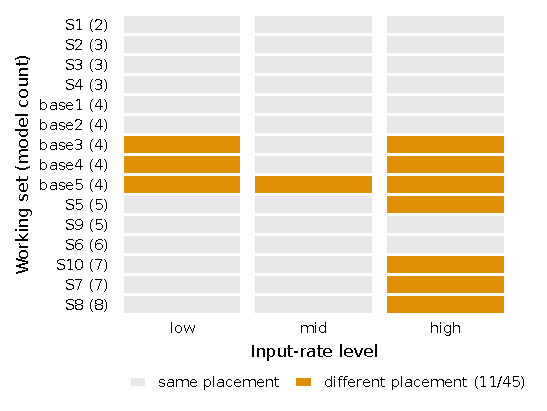
\includegraphics[width=0.66\linewidth]{fig_divergence.pdf}
\caption{Agreement between the GPU and NPU in their best measured placements at $\beta{=}1.0$. Orange cells indicate 11 disagreements, including 10 generative and one vision-only group.}
\label{fig:divergence}
\end{minipage}\hfill
\begin{minipage}[t]{0.40\linewidth}
\vspace{50pt}
\centering
\captionof{table}{Ranking quality on the shared measured candidate set under group-wise validation. The greedy baseline returns a single placement, so only Top-1 is reported and computed over measured outputs; the corresponding /45 lower bounds are 0.311 and 0.244.}
\label{tab:comparison}
\footnotesize
\setlength{\tabcolsep}{3pt}
\resizebox{\linewidth}{!}{%
\begin{tabular}{@{}l cc cc@{}}
\toprule
& \multicolumn{2}{c}{Spearman $\rho$} & \multicolumn{2}{c}{Top-1} \\
\cmidrule(lr){2-3}\cmidrule(lr){4-5}
Method & GPU & NPU & GPU & NPU \\
\midrule
Capacity greedy & --- & --- & 0.424 & 0.333 \\
Decomposed per instance & 0.931 & 0.911 & 0.911 & 0.622 \\
Direct regression & 0.986 & 0.972 & 0.933 & 0.867 \\
\midrule
Measured oracle & 1.00 & 1.00 & 1.00 & 1.00 \\
\bottomrule
\end{tabular}%
}
\end{minipage}
\end{figure}

\section{Methods Under Comparison}
\label{sec:methods}

We compare our direct model with two baselines and a measured oracle.

\textbf{Direct system-level regression.} Each placement is represented by features that summarize request rates, model types, device assignments, isolated device profiles, and aggregate load. Three XGBoost regressors~\citep{chen2016_xgboost} predict the normalized targets $\hat y_1$, $\hat y_2$, and $\hat y_3$. Equation~\eqref{eq:score} then converts these predictions into a ranking of candidate placements.

We use three-fold group-wise cross-validation. All placements from the same model-set--rate group remain in one fold. This protocol evaluates held-out rate-specific workload groups but does not require an entire model set and all of its rate levels to be absent from training. Targets are normalized within each group. Statistics from a held-out group are used only to construct its evaluation labels and never enter training. For the joint predictor, paired GPU and NPU samples from the same workload group are assigned to the same fold.


\textbf{Capacity greedy baseline.} This non-learning baseline uses the same request, placement, and isolated profile information as the predictor, but assumes that resource demand is additive. It considers instances in decreasing order of isolated accelerator speedup, admitting each one whose estimated load fits the remaining capacity budget; an instance that does not fit is placed on the CPU without stopping the scan. The VLM cannot run on the CPU and has the largest isolated accelerator speedup on both platforms; it is therefore admitted first, and its load is charged before any other instance.


\textbf{Decomposed per-instance model.}
This baseline adapts prior work on per-task degradation prediction~\citep{kim_iccd2024_interference}. A single shared regressor predicts the attainment of each vision instance under contention from its own configuration and a placement-level summary of its co-runners. Attainment is defined as achieved throughput divided by the smaller of the instance's request rate and isolated capacity. The instance-level predictions are composed into $\hat y_1$ and $\hat y_2$. For a conservative comparison, the composition step uses the measured normalization statistics of the evaluation group. This gives the decomposed baseline information that is unavailable to our direct predictor at deployment. The generative target $\hat y_3$ uses the same predictor as the direct model.

\textbf{Measured oracle.} The oracle selects the candidate with the highest measured score $S$ in each workload group and treats tied maxima as correct.

\section{Results}
\label{sec:results}

\textbf{Ranking quality.} Table~\ref{tab:comparison} summarizes ranking performance under group-wise validation. Our direct regression model achieves mean Spearman correlations of $0.986$ on the GPU and $0.972$ on the NPU. Top-1 accuracy is $0.933$ on the GPU and $0.867$ on the NPU, and the selected placement attains at least $91\%$ of the best measured score in every group (mean $99.6\%$/$99.3\%$). Per-set results are reported in Appendix~B. Unless otherwise noted, subsequent comparisons use the same validation protocol and measured candidate set.

\textbf{Best measured placements differ across accelerators.} Figure~\ref{fig:divergence} compares the best measured placement in each workload group. Under the normalized objective in Equation~\eqref{eq:score}, the GPU and NPU disagree on the best measured placement in 11 of 45 groups, including 10 of 33 generative groups and 1 of 12 vision-only groups. Reducing the generative weight to $\beta{=}0.5$ increases the number of disagreements to 16 of 45. Candidate sampling is unlikely to account for this result. Among the 30 exhaustively measured groups, 8 disagree across the two platforms. All 8 are generative, corresponding to 8 of 24 generative groups and none of the 6 vision-only groups. This divergence rate is no lower than that observed over the full candidate set. Sensitivity to the scoring coefficients is also asymmetric. With the generative term active ($\beta{>}0$), the GPU best measured placement changes in at most 3 of 15 workload sets across the sweep in Appendix~C, whereas the NPU best measured placement changes in up to 9 workload sets.

\textbf{Transfer across accelerators.}
Figure~\ref{fig:transfer} compares platform-specific, zero-shot, and joint training. The zero-shot predictor is trained on one accelerator and applied to the other without retraining or target co-execution data; features still use target-platform isolated profiles. The joint predictor is trained on pooled data from both platforms; it carries no explicit platform identifier; conditioning comes from device-assignment indicators and isolated-profile values. On the NPU, zero-shot transfer reduces Spearman correlation from $0.972$ to $0.902$ and Top-1 accuracy from $0.867$ to $0.800$. On the GPU, Spearman correlation decreases from $0.986$ to $0.927$, while Top-1 accuracy remains $0.933$. Joint training closes the gap. It reaches Spearman correlations of $0.975$ on the GPU and $0.984$ on the NPU, with Top-1 accuracies of $0.933$ and $0.867$---on the NPU matching the platform-specific Top-1 and exceeding its Spearman correlation.



\begin{figure}[t]
\centering
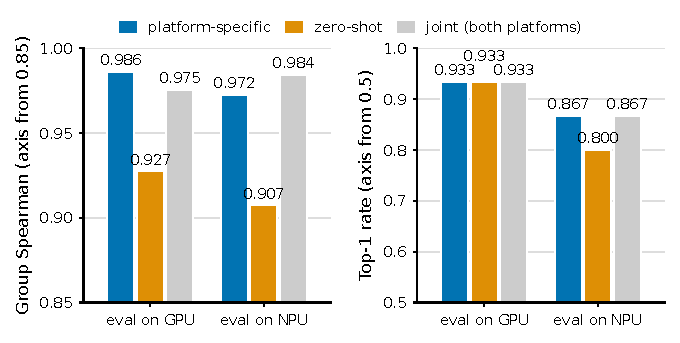
\includegraphics[width=2.4in]{fig_transfer.pdf}
\caption{Transfer under group-wise validation. Zero-shot degrades ranking, especially on the NPU; joint training approaches platform-specific performance. Axes start at $0.85$ (Spearman) and $0.5$ (Top-1).}
\vspace{-6pt}
\label{fig:transfer}
\end{figure}

\textbf{Comparison with simpler models.}
The capacity-based greedy baseline achieves Top-1 accuracies of $0.424$ on the GPU and $0.333$ on the NPU among outputs present in the measured candidate set. Because the greedy baseline uses the same request, placement, and isolated-profile inputs as direct regression, the performance gap indicates the benefit of learning nonadditive contention. Appendix~D compares two admission orderings for this baseline.

The decomposed model achieves pooled Spearman correlations of $0.993$ on the GPU and $0.992$ on the NPU for individual attainment prediction. However, its placement-level Top-1 accuracies fall to $0.911$ and $0.622$, respectively. Even when the deadline-miss target is reconstructed from measured attainments and group statistics, group-mean Spearman reaches only $0.877$ on the GPU and $0.720$ on the NPU, as reported in Appendix~E. For this attainment-based baseline, the main ranking loss arises from composing the instance-level estimates rather than predicting them. Under a set-level cluster bootstrap, the Top-1 advantage of direct regression over this baseline is significant on the NPU but not on the GPU (Appendix~H).


\section{Related Work}
\label{sec:related}
Cluster-scale serving systems optimize request scheduling rather than per-instance device assignment within a node~\citep{crankshaw_nsdi2017_clipper,shen_sosp2019_nexus,li_osdi2023_alpaserve,gujarati_osdi2020_clockwork}. Intra-node schedulers~\citep{oh_hpca2021_layerweaver,dagli_ppopp2024_haxconn,omniboost2025,yu2023partituner} operate at layer or operator granularity, which differs from our placement decision. Learned interference prediction is more closely related to our work. Abacus~\citep{cui2021} and iGniter~\citep{xu_tpds2023_igniter} target single-GPU overlap and provisioning, while \citet{kim_iccd2024_interference} train per-task interference models for runtime scheduling on a heterogeneous edge SoC with concurrent GPU/DLA execution. We instead study fixed pre-deployment CPU--accelerator placements across discrete GPU- and NPU-based platforms; our decomposed baseline adapts their per-task structure. HEFT assumes task-graph execution and communication costs, and RL-based placement learns from execution-derived rewards; our setting instead ranks fixed placements for streaming workloads from offline co-execution profiles~\citep{topcuoglu2002heft,mirhoseini2017_deviceplacement}.

\paragraph{Limitations and conclusion.}
Our evaluation is limited to the collected candidate placements; deployment on the stratified sets may rank unmeasured placements. Because $y_2$ is normalized within each workload group, it cannot certify absolute SLO satisfaction. The request-rate levels depend on workload-set size, which limits direct comparisons across sets. Dynamic re-placement is outside the scope of this study and could complement the offline placement method. Within these limits, best measured placements and profiling data are accelerator-specific. A single jointly trained predictor matches separately trained ones on both platforms, outperforms the capacity-based heuristic, and surpasses the attainment-based decomposition on the NPU.

\bibliographystyle{unsrtnat}
\bibliography{mlforsys_main}

\appendix
\section*{Appendix}


\subsection*{A. Candidate-set coverage by workload set} Training configuration and the full feature schema appear in Appendix~F. The feasibility rule that defines the candidate set is shared across profiling, evaluation, and deployment: a model may occupy any device its registry entry allows, and the VLM is pinned to the accelerator. Profiling additionally sub-samples the stratified sets to bound collection cost, whereas deployment enumerates the full feasible set; evaluation uses exactly the placements that were profiled.

This appendix characterizes the candidate-placement coverage for each workload set and examines whether the observed GPU--NPU placement divergence is an artifact of incomplete sampling.

The five workload sets labeled base1--base5 each contain LLaMA-3.2-1B, Qwen2-VL-2B, ResNet50, and one YOLO11 detector. They differ only in the detector variant, using YOLO11 n, s, m, l, and x, respectively. The remaining sets, S1--S10, vary in concurrency, generative-model composition, and request-rate configuration.

Table~\ref{tab:app_coverage} reports the full placement space, the feasible subset, and the measured subset for each workload set. Because each VLM is pinned to the accelerator, a set with $N$ instances has $2^{N-\#\mathrm{VLM}}$ feasible placements; sets without a VLM retain all $2^N$ placements. We measure ten workload sets exhaustively. For the remaining five, we stratify placements by the number of non-pinned instances assigned to the accelerator and sample each stratum using quotas fixed before data collection. Both platforms use the same generated measurement schedule, and post hoc verification confirms that their measured candidate sets are identical for every workload set and request-rate configuration.

All appendix analyses follow the normalization procedure in Section~2. Within each workload group, $y_1=r_1/\max r_1$ and $y_3=r_3/\max r_3$, while $y_2=(r_2-\min r_2)/(\max r_2-\min r_2)$, with $y_2{=}0$ when all candidates have the same $r_2$. We evaluate best measured placements with ties. Every candidate whose score is within $10^{-9}$ of the group maximum is included in the set of best measured placements. The two platforms are considered to agree when their sets of best measured placements intersect.

The sampling procedure does not explain the observed placement divergence. Among the 30 exhaustively measured workload groups, the GPU and NPU disagree on the best measured placement in 8 groups: 8 of 24 generative groups and none of the 6 vision-only groups. At $\beta{=}0.5$, 13 of the 30 exhaustive groups diverge. These rates are no lower than those obtained over all 45 groups. The sampled vision-only controls S9 and S10 account for only one divergence among their six workload groups, occurring for S10 at its highest request rate.

\begin{table}[h]
\centering
\caption{Placement-space coverage. Measured counts are identical on the
two platforms. Cov.\ = measured/feasible.}
\label{tab:app_coverage}
\footnotesize
\setlength{\tabcolsep}{5pt}
\begin{tabular}{@{}ll rrrr l@{}}
\toprule
Set & $N$ & $2^{N}$ & Feasible & Measured & Cov. & Mode \\
\midrule
S1  & 2 & 4   & 4   & 4  & 100\% & exhaustive \\
S2  & 3 & 8   & 8   & 8  & 100\% & exhaustive \\
S3  & 3 & 8   & 8   & 8  & 100\% & exhaustive \\
S4  & 3 & 8   & 4   & 4  & 100\% & exhaustive \\
base1--base5 & 4 & 16 & 8 & 8 & 100\% & exhaustive \\
S5  & 5 & 32  & 16  & 16 & 100\% & exhaustive \\
S9  & 5 & 32  & 32  & 16 & 50\%  & stratified \\
S6  & 6 & 64  & 32  & 16 & 50\%  & stratified \\
S7  & 7 & 128 & 64  & 20 & 31\%  & stratified \\
S10 & 7 & 128 & 128 & 24 & 19\%  & stratified \\
S8  & 8 & 256 & 128 & 24 & 19\%  & stratified \\
\bottomrule
\end{tabular}
\end{table}

\subsection*{B. Per-set out-of-fold ranking fidelity}
Table~\ref{tab:app_perset} reports per-target group Spearman correlations under the GroupKFold protocol, averaged across the request-rate levels of each workload set. The $y_3$ regressor is trained only on the 372 windows per platform in which a generative instance runs on the accelerator; the excluded 168 comprise 156 windows from vision-only workloads and 12 in which the LLM was placed on the CPU, whose CPU-only token rates are not usable labels. The trained regressor still scores every held-out candidate, and the $\beta$ term is applied per workload set rather than per placement, so these candidates compete in the ranking on equal footing; their extrapolated token-rate predictions do not change any reported result (all S3 groups rank correctly on both platforms). 

The $y_3$ metric applies only to sets containing a generative model. The two lowest values, observed for $y_3$ on S3-GPU and S4-NPU, come from $N{=}3$ sets with few valid $y_3$ candidates. A single rank inversion therefore changes the correlation substantially.

\begin{table}[h]
\centering
\caption{Per-set out-of-fold Spearman correlations, averaged over request-rate levels. A dash indicates that $y_3$ is not applicable.}
\label{tab:app_perset}
\footnotesize
\setlength{\tabcolsep}{4pt}
\begin{tabular}{@{}ll ccc ccc@{}}
\toprule
& & \multicolumn{3}{c}{GPU} & \multicolumn{3}{c}{NPU} \\
\cmidrule(lr){3-5}\cmidrule(lr){6-8}
Set & $N$ & $y_1$ & $y_2$ & $y_3$ & $y_1$ & $y_2$ & $y_3$ \\
\midrule
S1 & 2 & 1.000 & 0.811 & --- & 1.000 & 0.949 & --- \\
S2 & 3 & 0.992 & 0.820 & --- & 0.976 & 0.914 & --- \\
S3 & 3 & 0.992 & 0.894 & 0.400 & 0.881 & 0.837 & 0.867 \\
S4 & 3 & 0.933 & 0.867 & 0.933 & 0.867 & 0.966 & 0.533 \\
base1 & 4 & 1.000 & 0.892 & 0.960 & 0.929 & 0.932 & 0.960 \\
base2 & 4 & 1.000 & 0.922 & 0.929 & 0.968 & 0.980 & 0.968 \\
base3 & 4 & 0.984 & 0.984 & 0.976 & 0.992 & 0.956 & 0.952 \\
base4 & 4 & 1.000 & 0.968 & 0.984 & 0.992 & 0.946 & 0.960 \\
base5 & 4 & 0.968 & 0.960 & 0.992 & 0.976 & 0.889 & 0.992 \\
S5 & 5 & 0.995 & 0.929 & 0.976 & 0.951 & 0.883 & 0.973 \\
S9 & 5 & 0.993 & 0.930 & --- & 0.975 & 0.831 & --- \\
S6 & 6 & 0.984 & 0.977 & 0.972 & 0.973 & 0.966 & 0.973 \\
S10 & 7 & 0.997 & 0.931 & --- & 0.987 & 0.812 & --- \\
S7 & 7 & 0.993 & 0.954 & 0.950 & 0.980 & 0.935 & 0.964 \\
S8 & 8 & 0.998 & 0.944 & 0.974 & 0.981 & 0.958 & 0.973 \\
\bottomrule
\end{tabular}
\end{table}

\subsection*{C. Sensitivity to scoring coefficients}

Table~\ref{tab:app_sweep} evaluates how the best measured placements change as the scoring coefficients vary. For each $(\alpha,\beta)$ pair, it reports the number of workload sets whose best-measured set differs from the baseline at $\alpha{=}0.3$ and $\beta{=}1.0$. The comparison is tie-aware and covers all 15 workload sets.

When the generative objective is active with $\beta{>}0$, the two platforms exhibit different levels of sensitivity. The GPU best placement changes in at most three workload sets and, outside the low-$\alpha$ region, only S8 changes. In contrast, the NPU best placement changes in as many as nine sets, primarily among the base workloads, S5, and S7.

The $\beta{=}0$ setting removes the generative objective entirely and causes substantial changes on both platforms. We therefore include this setting for completeness but exclude it from the cross-platform sensitivity comparison. For any fixed $\beta{>}0$, varying only $\alpha$ changes the best placement in at most one set on the GPU and up to seven sets on the NPU. These results indicate substantially greater placement sensitivity on the NPU than on the GPU across the evaluated coefficient sweep.

\begin{table}[h]
\centering
\caption{Number of workload sets whose tie-aware best-measured set differs from the baseline at $\alpha{=}0.3$ and $\beta{=}1.0$, reported as GPU/NPU counts. The coefficient $\beta$ applies only to generative sets.}
\label{tab:app_sweep}
\footnotesize
\setlength{\tabcolsep}{6pt}
\begin{tabular}{@{}l ccccc@{}}
\toprule
& \multicolumn{5}{c}{$\beta$} \\
\cmidrule(lr){2-6}
$\alpha$ & 0 & 0.25 & 0.5 & 0.75 & 1.0 \\
\midrule
0.00 & 9/11 & 3/9 & 3/8 & 3/7 & 1/6 \\
0.15 & 4/10 & 3/7 & 3/6 & 1/4 & 1/4 \\
0.30 & 2/10 & 1/7 & 1/6 & 1/2 & 0/0 \\
0.45 & 1/10 & 1/7 & 1/5 & 1/2 & 1/2 \\
0.60 & 1/10 & 1/6 & 1/4 & 1/3 & 1/2 \\
\bottomrule
\end{tabular}
\end{table}



\subsection*{D. Greedy ordering variants and unmeasured placements}

Table~\ref{tab:app_greedy} compares the load-factor and speedup orderings. Oracle ratio is the mean, over groups with measured greedy outputs, of the ratio between the normalized score of the greedy-selected placement and the best normalized score in its group. This ratio can be negative when $y_1$ is near zero and the $-\alpha y_2$ term dominates. In the stratified-sampling sets S6--S10, a greedy ordering can produce a placement outside the measured candidate set. We exclude such outputs from the Top-1 evaluation rather than map them to nearby placements, and the reported denominators indicate the number of evaluable workload groups. Although the speedup ordering produces more unmeasured placements, it achieves higher measured-denominator Top-1 on both platforms; under the /45 lower bound, which counts every unmeasured output as incorrect, the advantage remains only on the NPU.

The two orderings also differ in when the VLM load is added to the capacity estimate. Under speedup ordering, the VLM is considered first, so its load is accounted for before any other admission decision. Under load-factor ordering, the VLM is considered only after one to three instances on the GPU and one to two instances on the NPU have already been admitted. This delayed accounting is more consequential on the NPU because the VLM consumes 0.13--0.40 of the estimated capacity, compared with 0.02--0.07 on the GPU. Since the VLM is admitted regardless of the remaining capacity, the cumulative estimated load exceeds 1.0 in 18 of the 45 NPU workload groups.

\begin{table}[h]
\centering
\caption{Capacity-based greedy performance under two admission orderings at $\alpha{=}0.3$ and $\beta{=}1.0$. Top-1 is evaluated only for measured outputs.}
\label{tab:app_greedy}
\footnotesize
\begin{tabular}{@{}ll ccc c@{}}
\toprule
Platform & Ordering & Top-1 (measured) & Top-1 (bound, /45) & Oracle ratio & Unmeasured \\
\midrule
GPU & load-factor & 0.341 (14/41) & 0.311 & 0.575 & 4/45 \\
GPU & speedup     & 0.424 (14/33) & 0.311 & 0.734 & 12/45 \\
NPU & load-factor & 0.250 (9/36)  & 0.200 & 0.590 & 9/45 \\
NPU & speedup     & 0.333 (11/33) & 0.244 & 0.793 & 12/45 \\
\bottomrule
\end{tabular}
\end{table}

\subsection*{E. Composition error in the decomposed model}

Table~\ref{tab:app_decomp} examines whether the performance loss of the decomposed model arises from per-instance prediction or from composing instance-level estimates into system-level metrics. The shared regressor predicts individual attainment accurately when all instance-level samples are pooled.

To isolate composition error, we reconstruct $y_2$ from measured rather than predicted attainments, thereby removing per-instance prediction error. The reconstruction also uses the measured group maximum for throughput normalization and the measured group minimum and maximum for deadline-miss normalization. These statistics are unavailable at deployment, so this analysis favors the decomposed baseline.

Despite these advantages, composing the measured attainments still reduces ranking fidelity. The aggregation rule does not account for request-rate weighting or interactions that are not represented in the individual instance views, including interference associated with a generative co-runner. The final row of Table~\ref{tab:app_decomp} reports the resulting placement-level ranking performance. Top-5 accuracy remains $1.000$ on both platforms, but the lower Top-1 accuracy shows that composition error affects identification of the best placement.


\begin{table}[h]
\centering
\caption{Error analysis of the decomposed model. Pooled metrics aggregate all instance-level samples, while group-mean $\rho$ averages rank correlations across workload groups.}
\label{tab:app_decomp}
\footnotesize
\resizebox{\linewidth}{!}{%
\begin{tabular}{@{}l cc@{}}
\toprule
Quantity & GPU & NPU \\
\midrule
Attainment OOF (pooled $\rho$ / MAE)
& $0.993 / 0.017$
& $0.992 / 0.020$ \\
Measured-attainment $y_2$ (pooled $\rho$ / group-mean $\rho$ / MAE)
& $0.834 / 0.877 / 0.149$
& $0.763 / 0.720 / 0.169$ \\
Composed ranking (group-mean $\rho$ / Top-1)
& $0.931 / 0.911$
& $0.911 / 0.622$ \\
\bottomrule
\end{tabular}%
}
\end{table}


\subsection*{F. Training configuration and feature schema}
For each outer fold and each target, $(\texttt{max\_depth}, \eta)$ is selected from a four-point grid---$(3, 0.1)$, $(4, 0.1)$, $(5, 0.05)$, $(6, 0.1)$---by an inner three-fold cross-validation split on the same workload groups as the outer folds, choosing the combination with the lowest mean absolute error; all other settings are fixed (squared-error objective, 300 boosting rounds, subsample and column-sample $0.8$, minimum child weight $3$, seed $42$). The same helper trains the platform-specific, joint, and decomposed models; the outer split is the three-fold group-wise protocol of Section~3.

Each placement is featurized from plan-level information only. Per instance, twelve values are computed: the assigned request rate (fps); three device-assignment indicators (CPU/GPU/NPU); two model-type indicators (vision, generative); four isolated-profile values for the assigned device---inference latency (ms), model load time (ms), token generation rate (tok/s; generative models only), and capacity ($1000/\mathrm{latency}$, fps); the load factor (request rate divided by capacity); and one interaction term (request rate $\times$ isolated latency). Aggregating each of the twelve values over all instances of a placement with sum, mean, and max yields 36 features; the instance count $N$ completes the 37-dimensional representation. The feature list is identical on both platforms; platform differences appear only in feature values. Execution settings and the software stack appear in Appendix~G.


\subsection*{G. Execution settings and software stack}
Both platforms share the host, schedules, and measurement procedure; only the accelerator path differs. Each window uses a 20\,s warm-up followed by a 180\,s measurement on a $1280{\times}720$ input video, with batch size~1 throughout and combination order randomized using seed~20260715. Vision models run at their native input sizes (YOLO11 at $640{\times}640$ letterbox; ResNet50 and MobileNet-v2 at $224{\times}224$) with single-threaded workers. On the GPU platform, vision models execute in FP32 via ONNX Runtime~1.20.1 with the CUDA execution provider; generative models run in FP16 (PyTorch~2.12). On the NPU platform, vision models execute as INT8-quantized compiled binaries on eight cores via the vendor model zoo, and generative models use vendor 8-bit-weight checkpoints (LLaMA on one core; the VLM uses one text core and four vision cores) under \texttt{mobilint-qb-runtime}~1.2.0. Generation uses greedy decoding with at most 64 (LLM) and 32 (VLM) new tokens, a fixed rotating prompt set for the LLM, and a fixed single prompt with one video frame for the VLM. Collection-time NVIDIA driver, CUDA/cuDNN build, and vendor compiler versions were not recorded and are omitted rather than reconstructed.


\subsection*{H. Robustness of the comparisons}
Uncertainty is estimated with a cluster bootstrap that resamples the 15 workload sets with replacement ($B{=}10{,}000$), keeping each set's three rate levels together. Table~\ref{tab:app_boot} reports 95\% percentile intervals for the headline metrics and for paired Top-1 differences computed on the same resamples. The advantages of direct regression over both greedy orderings, and over the decomposed baseline on the NPU, exclude zero; the GPU-side advantage over the decomposed baseline (one group) does not. The divergence fraction has a wide interval, reflecting the 15-set sample size.

\begin{table}[h]
\centering
\caption{Set-level cluster bootstrap (95\% percentile CIs). Greedy uses the /45 lower bound.}
\label{tab:app_boot}
\footnotesize
\setlength{\tabcolsep}{4pt}
\begin{tabular}{@{}l cc@{}}
\toprule
Quantity & GPU & NPU \\
\midrule
Direct group-mean Spearman & 0.986 [0.982, 0.990] & 0.972 [0.953, 0.986] \\
Direct Top-1 & 0.933 [0.867, 1.000] & 0.867 [0.756, 0.956] \\
Decomposed Top-1 & 0.911 [0.844, 0.978] & 0.622 [0.422, 0.800] \\
Divergence fraction (11/45) & \multicolumn{2}{c}{0.244 [0.089, 0.422]} \\
\midrule
Direct $-$ greedy (speedup) & +0.622 [+0.489, +0.756] & +0.622 [+0.422, +0.800] \\
Direct $-$ greedy (load-factor) & +0.622 [+0.489, +0.756] & +0.667 [+0.511, +0.800] \\
Direct $-$ decomposed & +0.022 [+0.000, +0.067] & +0.244 [+0.044, +0.467] \\
\bottomrule
\end{tabular}
\end{table}

\textbf{Divergence margins.} For each of the 11 disagreeing groups we compare, on each platform, the best measured score with the score that the other platform's best placement attains there. The smallest of the 22 margins is $2.6\times10^{-3}$ in normalized score---six orders of magnitude above the $10^{-9}$ tie width---and the median is $0.155$ (31\% of the median within-group score dispersion). Only two cells fall below $0.01$; under a coarser score-equivalence band of $0.01$, those two groups would count as agreeing and the divergence count would be 9 of 45. Because each placement was measured once, these margins do not quantify run-to-run uncertainty. Repeated measurements would be needed to establish a noise-aware equivalence threshold.

\textbf{Selected-placement quality.} Complementing Top-1, the ratio between the selected placement's measured score and the best measured score in its group averages $0.996$/$0.993$ (GPU/NPU) for direct regression, with a worst case of $0.921$/$0.910$ and no group below $0.9$. The decomposed baseline averages $0.980$/$0.951$ but with heavier tails (worst $0.249$/$0.455$; one and six groups below $0.9$). Greedy averages $0.734$/$0.793$ over measured outputs under speedup ordering, and $0.538$/$0.581$ when unmeasured outputs count as zero; under the normalized score this ratio can be negative.

\end{document}